% =========================================================
% METODOLOGÍA
% =========================================================

\chapter{Metodología Computacional}
\label{cap:metodologia}


% ---------------------------------------------------------
% Framework base
% ---------------------------------------------------------

\section{Framework Base: Modelado de Discos 1D}
\label{sec: tripodpy}
La evolución del disco protoplanetario se modeló utilizando \texttt{TriPoDPy} \citep{Pfeil2024_teoria, Kaufmann2025}, un framework desarrollado en Python que resuelve de manera acoplada la evolución viscosa del gas, el transporte radial del polvo y los procesos de coagulación y fragmentación en una dimensión radial. 

\invisiblesubsection{TriPoDPy y las Poblaciones de Polvo}

La resolución completa de la ecuación de coagulación de Smoluchowski \citep{Smoluchowski1916} resulta computacionalmente costosa. Para reducir este costo, \texttt{TriPoDPy} \citep{Pfeil2024_teoria, Kaufmann2025} aproxima la distribución local de tamaños mediante tres poblaciones características: granos pequeños ($a_0$), partículas intermedias ($a_1$) y pebbles correspondientes al tamaño máximo local ($a_{\rm max}$). Esta representación paramétrica permite describir la evolución del polvo con un costo computacional considerablemente menor.

\invisiblesubsection{Configuración Numérica y Condiciones Iniciales}

Las simulaciones se realizaron sobre una grilla radial logarítmica. Los parámetros globales y las configuraciones exploradas se resumen en la Tabla~\ref{tab:parametros_globales}.

\begin{table*}[t]
\centering
\caption{Parámetros globales del modelo. Los valores entre corchetes indican los rangos explorados en los barridos poblacionales.}
\small

\begin{tabular}{C{2.5cm}C{3.8cm}p{8.8cm}}
\hline\hline
Símbolo & Valor [Rango] & Descripción \\
\hline

\multicolumn{3}{c}{\textit{Estrella y disco}}\\
\hline

$M_*$ &
$1.0\,M_\odot$ &
Masa de la estrella central. \\

$R_*$ &
$2.1\,R_\odot$ &
Radio estelar inflado correspondiente a la fase de pre-secuencia principal. \\

$T_{\rm eff}$ &
$4000\,\mathrm{K}$ &
Temperatura efectiva que determina la estructura térmica del disco. \\

$M_{\rm disk}/M_*$ &
0.05 &
Fracción de masa inicial del disco. \\

$R_c$ &
$30.0\,\mathrm{AU}$ &
Radio característico asociado al decaimiento exponencial de la densidad superficial del gas. \\

$\alpha$ &
$10^{-3}\,[10^{-4}-10^{-2}]$ &
Parámetro de viscosidad turbulenta de Shakura--Sunyaev. \\

$R_{\rm in}-R_{\rm out}$ &
$0.5-100\,\mathrm{AU}$ &
Límites interno y externo del dominio radial. \\

$N_r$ &
300 &
Número de celdas de la grilla radial logarítmica. \\

\hline
\multicolumn{3}{c}{\textit{Embriones planetarios}}\\
\hline

$n_{\rm emb}$ &
1 &
Número de embriones por simulación. \\

$M_{\rm emb, 0}$ &
$10^{-4}\,M_\oplus\,[10^{-5}-10^{-2}]$ &
Masa inicial del embrión planetario. \\

$r_{\rm seed}$ &
$1.0\,\mathrm{AU}$ &
Ubicación radial del embrión. \\

\hline
\multicolumn{3}{c}{\textit{Gaps y subestructuras}}\\
\hline

$M_{\rm gap}$ &
$0.1\,M_{\rm Jup}\,[0.01-5.0]$ &
Masa del planeta gigante responsable de abrir el gap. \\

$r_{\rm gap}$ &
$10.0\,\mathrm{AU}\,[5.0-30.0]$ &
Ubicación radial del gap. \\

$A_{\rm sin}$ &
$[0.5-5.0]$ &
Amplitud de las perturbaciones sinusoidales. \\

\hline
\multicolumn{3}{c}{\textit{Línea de nieve y polvo}}\\
\hline

$v_{\rm frag}$ &
$1.0 \rightarrow 1.0-3.0-10.0\,\mathrm{m\,s^{-1}}$&
Velocidad umbral de fragmentación para silicatos en la región interior y hielos en la región exterior. \\

$r_{\rm SL}$ &
$\sim 2.7 \rightarrow 0.5\,\mathrm{AU}$ &
Evolución temporal de la posición de la línea de nieve. \\

\hline
\end{tabular}
\label{tab:parametros_globales}
\end{table*}


Finalmente, no se incorporó un modelo auto-consistente de evolución de la luminosidad estelar acoplado a la hidrodinámica del disco. La inclusión de un tratamiento termodinámico iterativo incrementaría significativamente el costo computacional de las simulaciones. Por esta razón, la evolución temporal de la \textit{snowline} se parametrizó de forma independiente, como se describe en la Sección~\ref{sec:snowline}. Esta aproximación permite reproducir de manera razonable la migración de la línea de nieve sin modificar la estructura hidrodinámica calculada por \texttt{TriPoDPy}.


% ---------------------------------------------------------
% Subestructuras
% ---------------------------------------------------------
\section{Implementación de Discos Estructurados}

Con el objetivo de modelar subestructuras asociadas a \textit{gaps} abiertos por planetas gigantes, se introdujeron perturbaciones locales en el parámetro de viscosidad turbulenta $\alpha$ de Shakura--Sunyaev \citep{Shakura_sunyaev_1973}. Los perfiles de gap se calcularon utilizando las parametrizaciones propuestas por \citet{Kanagawa2016} y \citet{Duffell2020}. En este trabajo se adoptó por defecto el modelo de \citet{Duffell2020}, ya que produce perfiles suaves y numéricamente estables, consistentes con simulaciones hidrodinámicas. Este enfoque permite que la estructura del disco se desarrolle de manera auto-consistente dentro del esquema viscoso resuelto por TriPoDPy \citep{Pfeil2024_teoria,Kaufmann2025}.


\invisiblesubsection{Implementación de los Pressure Bumps}

En lugar de modificar directamente la densidad superficial del gas ($\Sigma_{\rm gas}$) o del polvo ($\Sigma_{\rm dust}$), los \textit{gaps} se implementaron alterando localmente el parámetro de viscosidad turbulenta $\alpha$ de  \citet{Shakura_sunyaev_1973}. Este enfoque permite que la estructura del disco se desarrolle de manera auto-consistente dentro del esquema viscoso resuelto por \texttt{TriPoDPy}, evitando introducir discontinuidades artificiales en los perfiles de presión.

\invisiblesubsection{Evolución del Perfil de Densidad y Transporte de Sólidos}

La modificación local de $\alpha$ induce una redistribución de masa en el disco, generando gradientes de presión capaces de producir máximos locales de presión en el borde exterior del gap. Estas regiones pueden actuar como trampas de presión, reteniendo partículas sólidas y reduciendo el flujo radial de pebbles hacia las regiones internas del disco \citep{Pinilla2012, Kanagawa2016, Duffell2020}.

\begin{figure}[H]
    \centering
    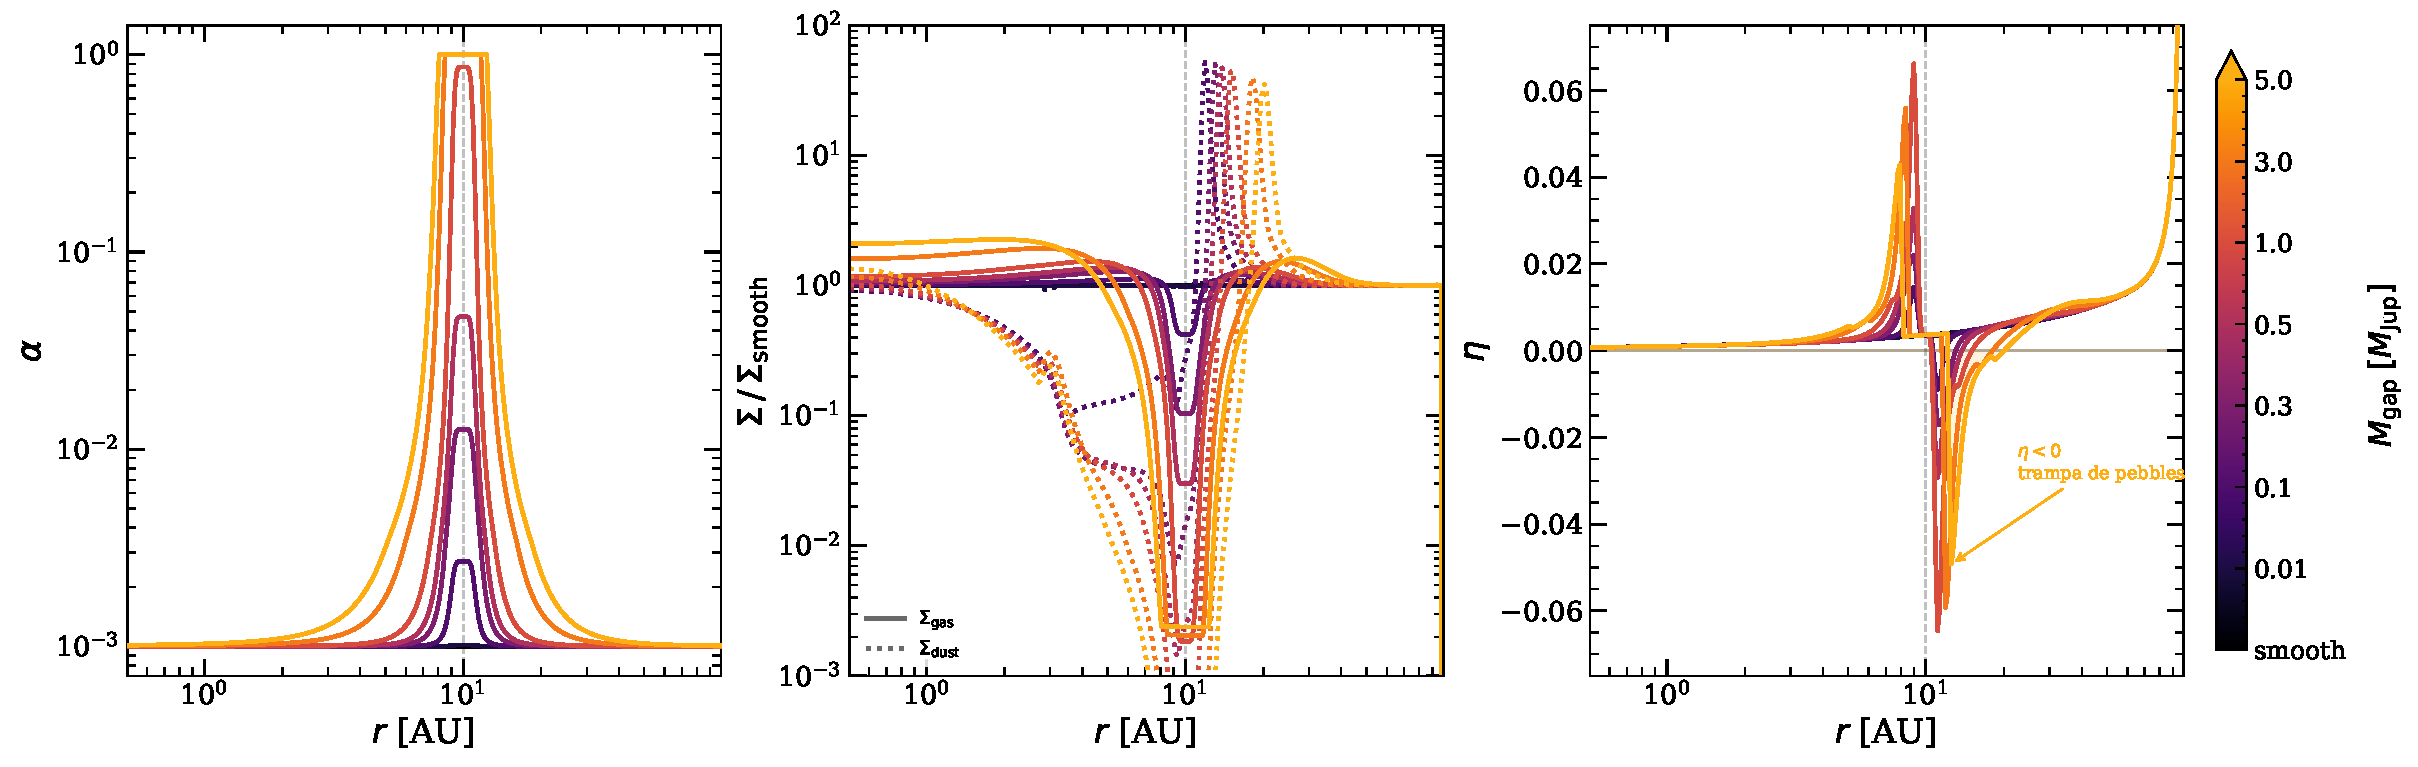
\includegraphics[width=1\linewidth]{figures/duffell_effect_panel.pdf}
    \caption{Perfiles radiales generados por la apertura de un \textit{gap} planetario según la parametrización de \citet{Duffell2020} para un valor base de $\alpha = 0.001$ e inyectando planetas con masas desde $M_{\text{gap}} = 0.01\,M_{\text{Jup}}$ hasta $5.0\,M_{\text{Jup}}$ (además del caso \textit{smooth} de control). \textbf{Panel izquierdo:} Perfil de la perturbación local aplicada sobre el parámetro de viscosidad turbulenta $\alpha(r)$. \textbf{Panel central:} Respuesta auto-consistente de la densidad superficial de gas ($\Sigma_{\text{gas}}$, líneas continuas) y polvo ($\Sigma_{\text{dust}}$, líneas punteadas) normalizadas respecto al perfil suave ($\Sigma/\Sigma_{\text{smooth}}$). \textbf{Panel derecho:} Modificación del parámetro $\eta(r)$; el cruce hacia valores negativos ($\eta < 0$) explicita la formación de la trampa de \textit{pebbles} en el borde externo de la subestructura.}
    \label{fig:duffel_efect_panel}
\end{figure}



Además, en \texttt{TriPoDPy} el parámetro $\alpha$ controla tanto la mezcla vertical y radial como las velocidades relativas entre partículas. En consecuencia, regiones menos turbulentas presentan velocidades de colisión más bajas, favoreciendo el crecimiento de partículas de mayor tamaño y números de Stokes más elevados.


% ---------------------------------------------------------
% Snowline dinámica
% ---------------------------------------------------------

\section{Evolución Dinámica de la Snowline}
\label{sec:snowline}

La línea de nieve del agua (\textit{water snowline}) corresponde a la región del disco protoplanetario donde la temperatura desciende por debajo de $\sim150-170,\mathrm{K}$, permitiendo la condensación del vapor de agua y la formación de mantos de hielo sobre las partículas sólidas \citep{Oka2011, Banzatti2023}. Esta transición modifica tanto las propiedades físicas del polvo como la composición de los pebbles disponibles para acreción planetaria \cite{}.

\invisiblesubsection{Evolución Temporal de la Tasa de Acreción}

A medida que el disco evoluciona, la disminución de la tasa de acreción estelar reduce el calentamiento viscoso y produce un enfriamiento progresivo del disco. Para describir esta evolución se adoptó una parametrización semianalítica basada en la ley de decrecimiento propuesta por \citet{Hartmann1998}, combinada con los modelos radiativos de \citet{Oka2011}. De acuerdo con \citet{Hartmann1998}, la tasa de acreción en estrellas de pre-secuencia principal decrece aproximadamente como

\begin{equation}
\dot{M}_\star \propto t^{-\eta}
\end{equation}

donde se adoptó un índice $\eta=1.5$. Asimismo, se utilizó como condición de referencia una tasa de acreción típica de $\dot{M}_\star \approx 10^{-8}M_\odot \mathrm{yr^{-1}}$ a una edad de $1\mathrm{Myr}$, característica de sistemas tipo T-Tauri. Esta parametrización permitió reconstruir la evolución temporal de la tasa de acreción a lo largo de varios millones de años (Figura~\ref{fig:hartmann_mdot}).

\begin{figure}[H]
    \centering
    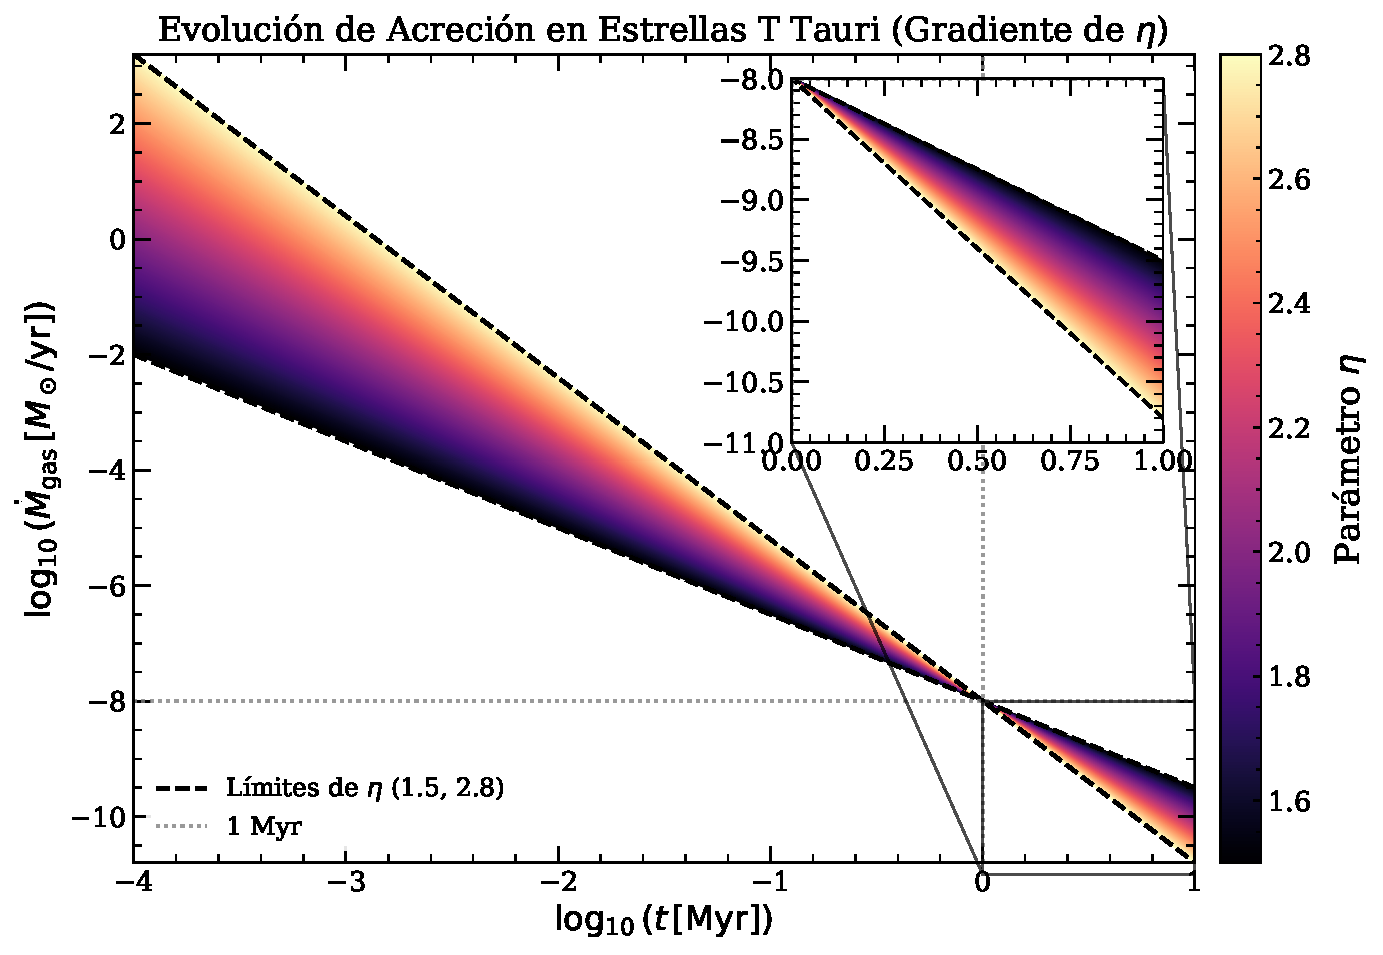
\includegraphics[width=0.8\textwidth]{figures/hartmann_mdot_gradient.pdf}
    \caption{Evoluci\'on param\'etrica de la tasa de acreci\'on de gas ($\dot{M}_{\text{gas}}$) en funci\'on del tiempo para estrellas T Tauri, basada en el modelo anal\'itico de \citet{Hartmann1998}. El eje vertical representa el logaritmo de la tasa de acreci\'on en $M_{\odot}\,\text{yr}^{-1}$, y el eje horizontal el logaritmo del tiempo en Myr. La regi\'on sombreada ilustra una familia de soluciones donde la barra de color indica el valor del exponente de decaimiento $\eta$, variando continuamente desde $1.5$ (tonos oscuros) hasta $2.8$ (tonos claros). Las l\'ineas discontinuas negras delimitan las cotas superior e inferior correspondientes a estos valores extremos de $\eta$. Se incluye una l\'inea punteada de referencia marcando el tiempo $t = 1\text{ Myr}$ ($\log_{10} t = 0$). El recuadro interior (\textit{inset}) muestra una vista ampliada de la etapa de evoluci\'on tard\'ia ($t \geq 1\text{ Myr}$), destacando la divergencia en la ca\'ida de la tasa de acreci\'on dependiente del par\'ametro $\eta$.}
    \label{fig:hartmann_mdot}
\end{figure}

Los valores temporales de la tasa de acreción se combinaron con los perfiles de temperatura y posición de la snowline obtenidos por \citet{Oka2011} (Figura~\ref{fig:dynamic_snowline}). A partir de esta información se construyó una parametrización de la evolución temporal de $R_{\rm snow}(t)$ mediante interpolación, permitiendo describir la migración de la línea de nieve a lo largo de la evolución del disco.

Para las etapas más tempranas ($t \lesssim 0.2,\mathrm{Myr}$), correspondientes a tasas de acreción elevadas ($\dot{M}_{gas} \gtrsim 10^{-7},M\odot,\mathrm{yr}^{-1}$), los valores se encuentran fuera del rango cubierto por los modelos de \citet{Oka2011}. En consecuencia, se asumió que la línea de nieve permanecía aproximadamente constante en $R_{\rm snow}\simeq2.7,\mathrm{AU}$ hasta que la disminución de la tasa de acreción permitió el inicio de su migración hacia el interior del disco.


\begin{figure}[H]
    \centering
    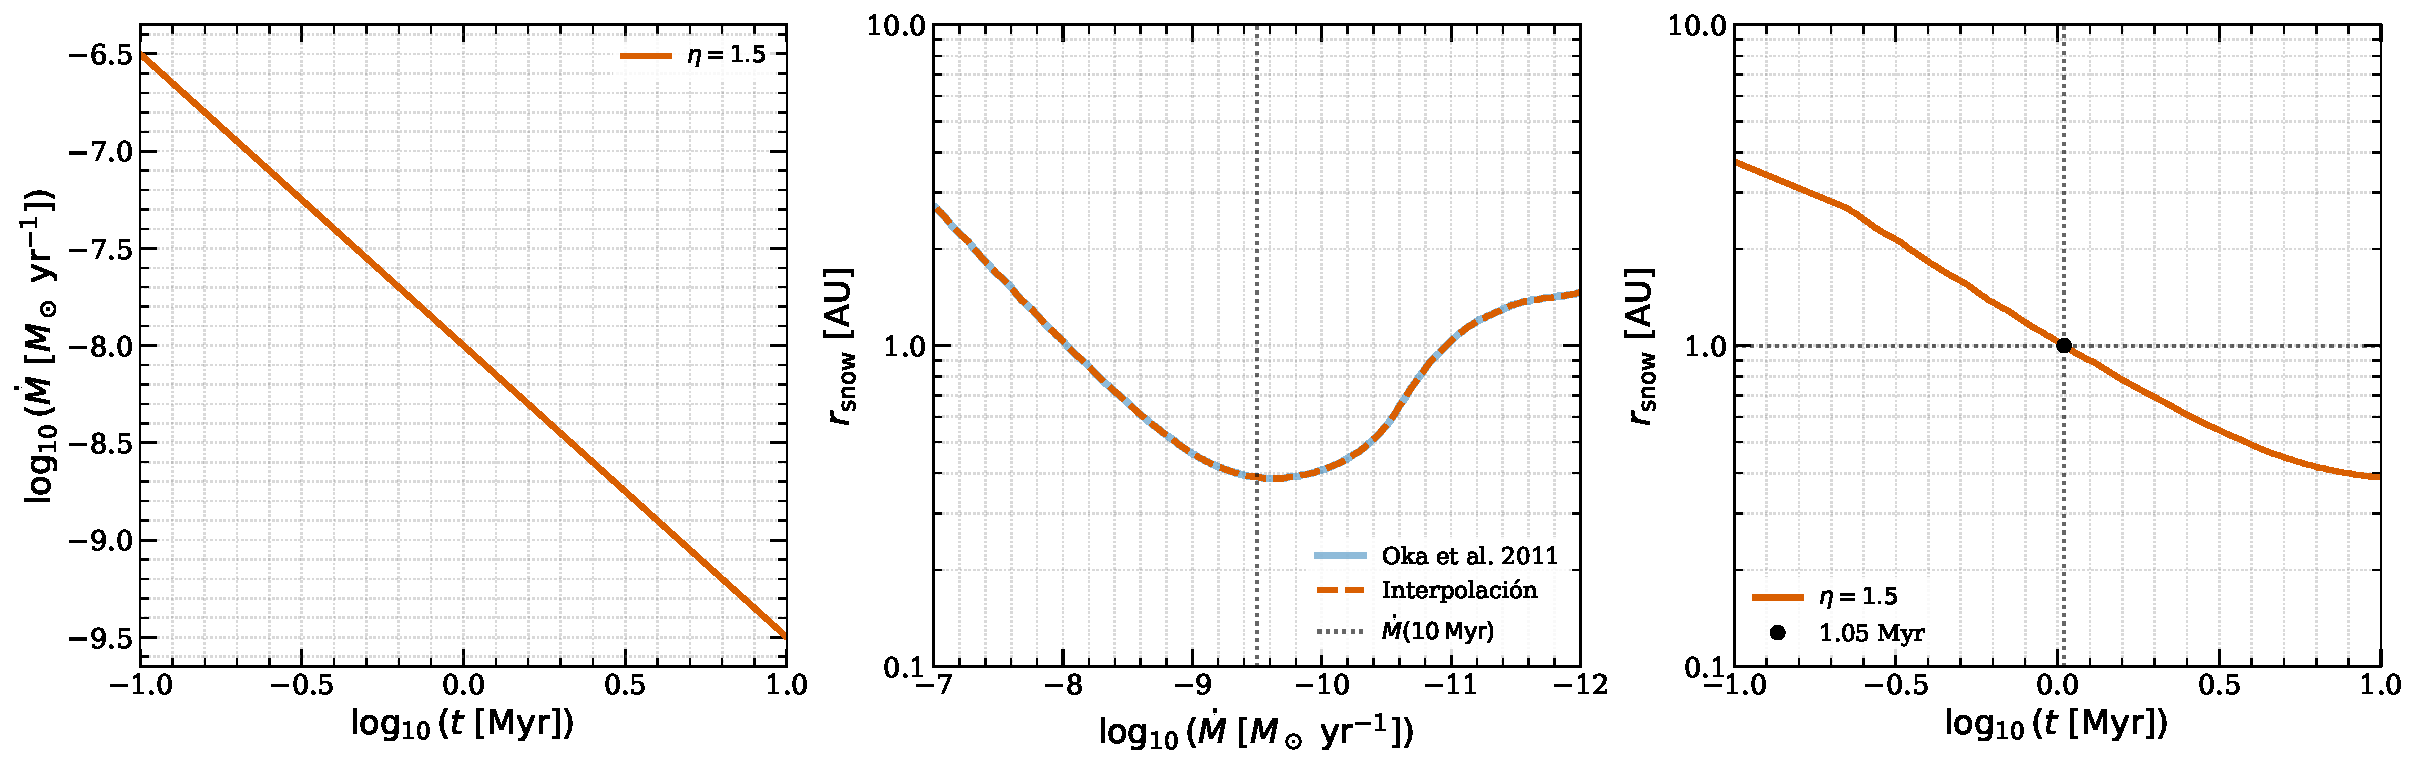
\includegraphics[width=1\textwidth]{figures/dynamic_snowline_oka_interpolation.pdf}
    \caption{Evoluci\'on din\'amica de la posici\'on de la l\'inea de nieve (\textit{snowline}) en la simulaci\'on base. 
    \textbf{Panel izquierdo:} Decaimiento temporal de la tasa de acreci\'on de gas ($\dot{M}$) asumiendo un modelo param\'etrico con exponente $\eta = 1.5$ \citep{Hartmann1998}. 
    \textbf{Panel central:} Dependencia te\'orica del radio de la \textit{snowline} ($r_{\text{snow}}$) respecto a la tasa de acreci\'on. Se muestra el modelo anal\'itico de \citet{Oka2011} (l\'inea s\'olida celeste) junto con la interpolaci\'on aplicada en este trabajo (l\'inea discontinua naranja). El eje horizontal ($\log_{10}\dot{M}$) se ha invertido intencionalmente para que la evoluci\'on temporal fluya hacia la derecha. La l\'inea vertical punteada sirve de referencia para la tasa de acreci\'on a los $10\text{ Myr}$. 
    \textbf{Panel derecho:} Trayectoria final de la \textit{snowline} acoplando las dos relaciones anteriores en funci\'on del tiempo astrof\'isico. El marcador negro y las l\'ineas punteadas transversales resaltan el momento exacto en el que la \textit{snowline} retrocede cruzando la marca de $1.0\text{ AU}$, lo cual ocurre a los $1.05\text{ Myr}$.}
    \label{fig:dynamic_snowline}
\end{figure}

\invisiblesubsection{Fragmentación Dependiente de la Composición Hielo-Roca}

La velocidad de fragmentación $v_{\rm frag}$ constituye uno de los parámetros más importantes en la evolución del polvo, ya que determina el tamaño máximo alcanzado por los pebbles y, en consecuencia, controla tanto sus velocidades de deriva radial como la eficiencia del transporte de sólidos. En este trabajo se adoptó una parametrización dependiente de la posición de la \textit{snowline}, implementada mediante una función escalón:
\begin{equation} v_{\rm frag}(r,t) = \begin{cases} 10 \, \text{m/s} & \text{si } r \geq R_{\rm snow}(t) \quad \text{(Material pegajoso rico en hielos)} \\ 1 \, \text{m/s} & \text{si } r < R_{\rm snow}(t) \quad \text{(Matriz rígida seca de silicatos)} \end{cases} \end{equation}
donde los valores exteriores representan agregados ricos en hielo y los interiores corresponden a partículas dominadas por silicatos. Esta prescripción se basa en experimentos de laboratorio que muestran que la presencia de hielo aumenta significativamente la resistencia a la fragmentación, permitiendo velocidades críticas del orden de \SI{10}{\meter\per\second}

Si bien estudios más recientes sugieren que la resistencia mecánica del hielo puede disminuir a temperaturas muy bajas, alcanzando valores comparables a los de los silicatos
(\SIrange{1}{3}{\meter\per\second}) \citep{Musiolik_Grzegorz_Gerhard2019}, en esta tesis se adoptó la aproximación estándar utilizada en modelos de evolución de polvo y formación planetaria. Bajo esta prescripción, valores elevados de $v_{\rm frag}$ favorecen la formación de pebbles de mayor tamaño, los cuales experimentan una deriva radial más eficiente y pueden modificar significativamente el flujo de sólidos hacia las regiones internas del disco.


% ---------------------------------------------------------
% Pebble Accretion
% ---------------------------------------------------------
\section{Modelo Computacional de Acreción: \texttt{PA3Py}}
\label{sec: PA3Py}

\texttt{PA3Py}\footnote{El código fuente completo de PA3Py, incluyendo 
documentación y tutoriales, está disponible públicamente en: 
\url{https://github.com/maximiliano-valderrama/pa3py}. El repositorio 
incluye además los datos de las 5006 trayectorias simuladas, scripts 
de análisis y figuras suplementarias para robustez a variaciones en 
$M_{\rm emb,0}$.} es el módulo de postprocesado desarrollado en este trabajo para estudiar el crecimiento de embriones planetarios mediante pebble accretion. El código implementa numéricamente las ecuaciones descritas en la Sección~\ref{sec:pebble_accretion} del Capítulo~\ref{cap:marco_teorico}, incluyendo los distintos regímenes de acreción (2D y 3D), así como las masas características asociadas al inicio de la acreción y al aislamiento por pebbles.

La evolución temporal se calcula mediante un esquema explícito de Euler utilizando como entrada los \textit{snapshots} en formato HDF5 generados por \texttt{TriPoDPy}. Para cada instante, el código extrae las propiedades locales del disco, incluyendo la densidad superficial del gas y del polvo, la temperatura, la altura de escala y las distribuciones de tamaño representadas por las poblaciones características ($a_0$, $a_1$ y $a_{\rm max}$).

\invisiblesubsection{Regímenes de Acreción}

Durante la integración, se introducen embriones planetarios de masa inicial $M_c$ en radios orbitales prefijados y se calcula su crecimiento siguiendo la formulación presentada por \citet{Ormel2017} y \citet{Drazkowska2023}. En primer lugar, se verifica que la masa del embrión supere la masa mínima necesaria para que la acreción de pebbles sea eficiente, conocida como \textit{onset mass},

\begin{equation}
M_{\rm PA,onset}=St\text{ }\eta^3\text{ }M_\star 
\end{equation}

donde $St$ es el número de Stokes y $\eta$ cuantifica la desviación sub-Kepleriana del gas. Para masas inferiores a este umbral, el crecimiento está dominado por colisiones geométricas y resulta poco eficiente.

Una vez superada esta condición, la acreción se calcula utilizando las expresiones correspondientes a los regímenes bidimensionales dominados por \textit{headwind} o (\textit{shear}), de acuerdo con las ecuaciones presentadas por \citet[][Ecs. 7.9 y 7.13]{Ormel2017}.

\invisiblesubsection{Corrección por Espesor Vertical}

En regiones donde la altura de la capa de pebbles excede el radio efectivo de captura gravitacional, el crecimiento se reduce mediante la corrección de transición suave propuesta por \citet[][Ec. 7.24]{Ormel2017}. Este factor permite describir la transición entre los regímenes 2D y 3D y tiene en cuenta la distribución vertical del polvo en el disco.

\invisiblesubsection{Masa de Aislamiento}

El crecimiento por pebble accretion se detiene cuando el planeta alcanza la masa de aislamiento,

\begin{equation}
M_{\rm iso}\approx25,M_\oplus
\left(\frac{H_{\rm gas}/r}{0.05}\right)^3
\frac{M_\star}{M_\odot},
\label{eq: Mass_isolation}
\end{equation}

siguiendo la aproximación adoptada por \citet{Lambrechts2014} y \citet{Drazkowska2023}. A esta masa, las perturbaciones gravitacionales inducidas por el planeta modifican localmente el perfil de presión del gas, generando una barrera que interrumpe el flujo radial de pebbles y detiene el crecimiento posterior mediante este mecanismo.


Una limitación del enfoque de \textit{post-procesado} radica en que \texttt{PA3Py} utiliza las propiedades del disco obtenidas por \texttt{TriPoDPy} sin retroalimentar su evolución. Por ello, la masa acrecida por un planeta no se descuenta del reservorio de sólidos disponible para otros cuerpos. Como resultado, simulaciones con múltiples planetas no incluyen la competencia por el flujo de pebbles, lo que puede producir una sobreestimación de la masa total acumulada.

\invisiblesubsection{Seguimiento Composicional del Contenido de Agua}

Para seguir la composición del material acrecido, se incorporó una contabilidad sencilla basada en la posición de origen de los pebbles respecto de la snowline. De manera consistente con trabajos previos \citep{Bitsch2021,McCloat2025}, se asumió que los pebbles formados más allá de la línea de nieve ($r \geq R_{\rm snow}(t)$) están compuestos por un 50\% de material refractario y un 50\% de hielo de agua, mientras que aquellos provenientes de regiones interiores se consideraron completamente secos. A partir de esta prescripción se calculó la evolución temporal del contenido de agua de cada planeta.


% ---------------------------------------------------------
% Resultados y Validación
% ---------------------------------------------------------
\section{Resultados y Validación de Simulaciones}

\invisiblesubsection{Configuración del Disco y Estructura Termodinámica}

Para este estudio, se generaron un total de 1323 simulaciones de disco físico bidimensionales, abarcando distintas configuraciones de subestructuras. Estas incluyen discos de control sin perturbaciones (\textit{Smooth}, 24 casos), discos con un único \textit{gap} (759 casos) y \textit{Sinusoidal} (540 casos).

Un aspecto fundamental de estas simulaciones es la suposición de un perfil térmico estático. Dado que la altura de escala de presión del gas obedece la proporcionalidad matemática
\begin{equation}
\frac{H_p}{r} \propto T^{1/2} r^{1/2} M_\star^{-1/2},
\end{equation}
y considerando que la masa estelar se asume constante en $1\,M_\odot$, el perfil de temperatura impuesto fija una estructura termodinámica invariante para el gas de fondo. El análisis de las simulaciones confirmó empíricamente que a $1\,{\rm AU}$, la razón de aspecto del disco gaseoso resulta idéntica en todas las simulaciones, arrojando un valor de $H_p/r \simeq 0.027$. 

Esta constancia termodinámica tiene implicaciones directas sobre el crecimiento de los núcleos. Recordando la expresión teórica para la masa de aislamiento inducida por el flujo de \textit{pebbles} \eqref{eq: Mass_isolation} y evaluando con el valor derivado de $H_p/r \simeq 0.027$, se obtiene una masa máxima teórica de $M_{\rm iso} \simeq 3.96\,M_\oplus$ a $1\,{\rm AU}$. Por lo tanto, la estructura del gas actúa como un escenario estático que impone una cota de masa al crecimiento de los embriones.

\invisiblesubsection{Inyección de Embriones}

Sobre esta colección de 1323 simulaciones de discos, se realizó un barrido exhaustivo del espacio de parámetros inyectando embriones planetarios con cuatro masas iniciales distintas: $M_{\rm emb,0} = 10^{-5},\; 10^{-4},\; 10^{-3},\; 10^{-2}\,M_\oplus$. Este procedimiento arrojó un catálogo total de 5292 trayectorias evolutivas planetarias únicas.

Con el fin de garantizar la consistencia numérica de la muestra, se aplicó un procedimiento de control de calidad sobre las 5292 trayectorias. Se definieron dos criterios principales de exclusión:

\begin{itemize}
    \item \textbf{Muerte prematura:} Simulaciones que finalizaron antes de alcanzar $1\,{\rm Myr}$ sin acumular al menos el $90\%$ de la masa de aislamiento esperada.
    \item \textbf{Inestabilidad numérica:} Integraciones que presentaron variaciones abruptas de masa en los últimos pasos temporales ($R_{\rm var} \geq 10\%$).
\end{itemize}

La aplicación de estos criterios condujo a la eliminación de aproximadamente 286 simulaciones ($\approx 5.4\%$ de la muestra), equivalente a $\sim 71$ casos por cada valor de $M_{\rm emb,0}$. Tras esta depuración, se obtuvo una muestra final de 5006 trayectorias válidas, empleadas en todos los análisis posteriores.

